
\serie{Perspective cavalière}

\begin{exercice}[Solides en vrac]
\begin{colenumerate}{2}
 \item
 
 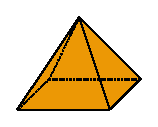
\includegraphics[width=2.3cm]{perspcav_orange}
 \item
 
 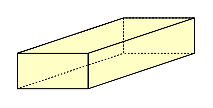
\includegraphics[width=3.2cm]{perspcav_beige}
 \item
 
 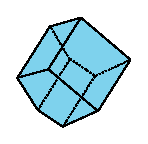
\includegraphics[width=2cm]{perspcav_bleu}
 \item
 
 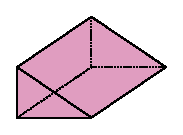
\includegraphics[width=2.7cm]{perspcav_rose}

 \end{colenumerate}
Pour chacun des solides, donne le nombre de sommets, d'arêtes et de faces. 
\end{exercice}


\begin{exercice}[Parallélépipède rectangle] \label{VolSol_entrain2}
Voici la représentation en perspective cavalière d'un parallélépipède rectangle $ABCDEFGH$ :
\begin{center} 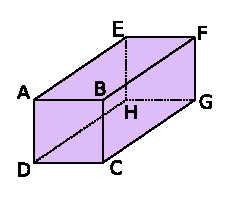
\includegraphics[width=3cm]{parallrect_violet} \end{center}
\begin{enumerate}
 \item Donne deux autres noms possibles pour ce pavé droit.
 \item Combien a‑t‑il de sommets ? Nomme‑les.
 \item Donne le nombre de faces puis nomme‑les.
 \item Combien d'arêtes a‑t‑il ? Nomme‑les.
 \item Nomme les arêtes qui ne sont pas visibles.
 \end{enumerate}
\end{exercice}


\begin{exercice}[Avec un cube] \label{VolSol_entrain1}
Soit le cube $POINTUES$ représenté ci‑dessous :
\begin{center} 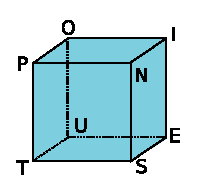
\includegraphics[width=2.6cm]{pointues} \end{center}
\begin{enumerate}
 \item Donne le nombre de sommets, le nombre d'arêtes et le nombre de faces de ce cube.
 \item Quelle est la nature de la face $PNST$ ?
 \item Quelle est la nature de la face $POIN$ ?
 \item Quelles sont les faces cachées du cube ?
 \end{enumerate}
\end{exercice}


\begin{exercice}[Avec un cube (bis)]
La représentation en perspective cavalière du cube $POINTUES$ est à l'exercice \ref{VolSol_entrain1}.
\begin{enumerate}
 \item Nomme la (ou les) face(s) parallèle(s) à la face $POIN$ ;
 \item Nomme la (ou les) face(s) perpendiculaire(s) à la face $PNST$ ;
 \item Cite toutes les arêtes de même longueur que l'arête $[PO]$ ;
 \item Combien d'arêtes ne sont pas visibles ? Nomme‑les ;
 \item Si on pose ce cube sur la face $NIES$, les faces $POIN$ et $OUEI$ étant visibles, quelles sont alors les faces cachées de ce cube ?
 \end{enumerate}
\end{exercice}


\begin{exercice}[Longueurs]
Soit le pavé droit $ABRICOTS$ tel que $AB = 3\,\text{cm}$, $BR = 4\,\text{cm}$ et $AC = 6\,\text{cm}$ :
\begin{enumerate}
 \item Fais, à main levée, une représentation en perspective cavalière de ce pavé droit. Code les arêtes de même longueur sur ton dessin.
 \item Recopie et complète le tableau :
 \begin{center}
  \begin{tabularx}{\linewidth}{|c|*{6}{>{\centering\arraybackslash}X|}}
  \hline
  \cellcolor{C3} Arêtes & \cellcolor{A4} $[IR]$ & \cellcolor{J4} $[BO]$ & \cellcolor{A4} $[CS]$ & \cellcolor{J4} $[RT]$ & \cellcolor{A4} $[CO]$ & \cellcolor{J4} $[OT]$ \\\hline
  \cellcolor{C3} Longueur & \cellcolor{A4} & \cellcolor{J4} & \cellcolor{A4} & \cellcolor{J4} & \cellcolor{A4} & \cellcolor{J4} \\
  \cellcolor{C3} (en cm) & \cellcolor{A4} & \cellcolor{J4} & \cellcolor{A4} & \cellcolor{J4} & \cellcolor{A4} & \cellcolor{J4} \\\hline
  \end{tabularx}
  \end{center}
 \vspace{0.3cm}
 \item Trace en vraie grandeur les faces $ABRI$ et $ABOC$.
 \item En utilisant la figure précédente, donne une valeur approchée de la longueur $BC$.
 \end{enumerate}
\end{exercice}


\begin{exercice}[Vrai / Faux]
On considère le pavé droit de l'exercice \ref{VolSol_entrain2}. Pour chaque affirmation, indique si elle est vraie ou fausse :
\begin{enumerate}
 \item Les faces $ABCD$ et $EFGH$ sont parallèles ;
 \item La face $ABCD$ est un carré ;
 \item L'angle $\widehat{GHD}$ mesure $120^\circ$ environ ;
 \item $ABC$ est un triangle rectangle et isocèle en $B$ ;
 \item L'angle $\widehat{BEF}$ mesure moins de $90^\circ$ ;
 \item L'angle $\widehat{ABF}$ est un angle droit ;
 \item Les arêtes $[AB]$ et $[BF]$ sont parallèles ;
 \item Les arêtes $[EH]$ et $[BF]$ sont sécantes ;
 \item Les arêtes $[CG]$ et $[FG]$ ne sont pas perpendiculaires ;
 \item La face $ADHE$ est un rectangle.
 \end{enumerate}
\end{exercice}


\begin{exercice}[Perspective et pavé droit]
Un parallélépipède rectangle a pour dimensions 2 cm ; 4,5 cm et 5,5 cm :
\begin{enumerate}
 \item Réalise à main levée une représentation possible de ce pavé droit en perspective cavalière puis code ton dessin ;
 \item Construis, à l'aide des instruments de géométrie, une représentation en perspective cavalière de ce pavé droit.
 \end{enumerate}
\end{exercice}


\begin{exercice}[Perspective et cube]
Un cube a une arête de 5 cm :
\begin{enumerate}
 \item À main levée, dessine ce cube en perspective cavalière puis code ton dessin ;
 \item Construis, sur papier quadrillé, une représentation en perspective cavalière de ce cube.
 \end{enumerate}
\end{exercice}


\begin{exercice}
On empile deux cubes identiques d'arête 2 cm l'un sur l'autre :
\begin{enumerate}
 \item Décris le solide obtenu et donne ses dimensions ;
 \item Représente ce solide en perspective cavalière sur papier quadrillé.
 \end{enumerate}
\end{exercice}


\begin{exercice}[Perspective sur quadrillage]
Reproduis puis complète les dessins suivants pour obtenir des représentations en perspective cavalière d'un pavé droit :
\begin{center} 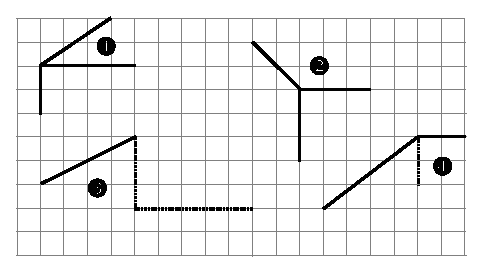
\includegraphics[width=8cm]{persp_quadrillage} \end{center}
\end{exercice}


\begin{exercice}[Araignée]
\begin{minipage}[c]{0.52\linewidth}
Une araignée part du sommet $F$ pour aller au sommet $E$. Elle ne marche que sur les arêtes de ce pavé droit :
 \end{minipage} \hfill%
 \begin{minipage}[c]{0.44\linewidth}
  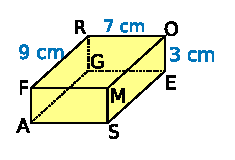
\includegraphics[width=3.5cm]{parcours_araignee}
  \end{minipage} \\
\begin{enumerate}
 \item Quel est le chemin le plus court ? Y a‑t‑il plusieurs possibilités ? Si oui, donne‑les toutes.
 \item Calcule la longueur de ce chemin.
 \end{enumerate}
\end{exercice}


\begin{exercice}[Empilements]
Le solide ci‑dessous est composé de cubes ayant pour arête 3 cm. La face du bas, la face arrière et la face de gauche sont des carrés :
\begin{center} 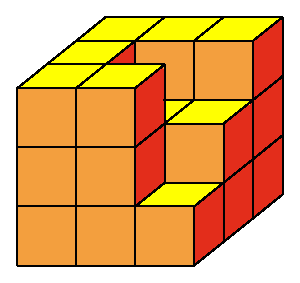
\includegraphics[width=4.7cm]{empilements} \end{center}
\begin{enumerate}
 \item Combien de cubes faudrait‑il ajouter pour obtenir un cube d'arête 9 cm ?
 \item Combien de cubes contient ce solide ?
 \item Dessine en vraie grandeur la face de dessus et la face de droite.
 \end{enumerate}
\end{exercice}


\begin{exercice}[Paquets]
Mandy veut ficeler des paquets de dimensions 20 cm, 15 cm et 50 cm. Elle a besoin de 25 cm par paquet pour faire le nœud. Mandy possède deux pelotes de ficelle de 95 m chacune.
\begin{colenumerate}{2}
 \item
 
 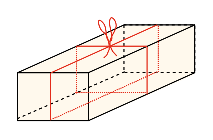
\includegraphics[width=3.1cm]{pelote1} \label{VolSol_entrain3}
 \item
 
 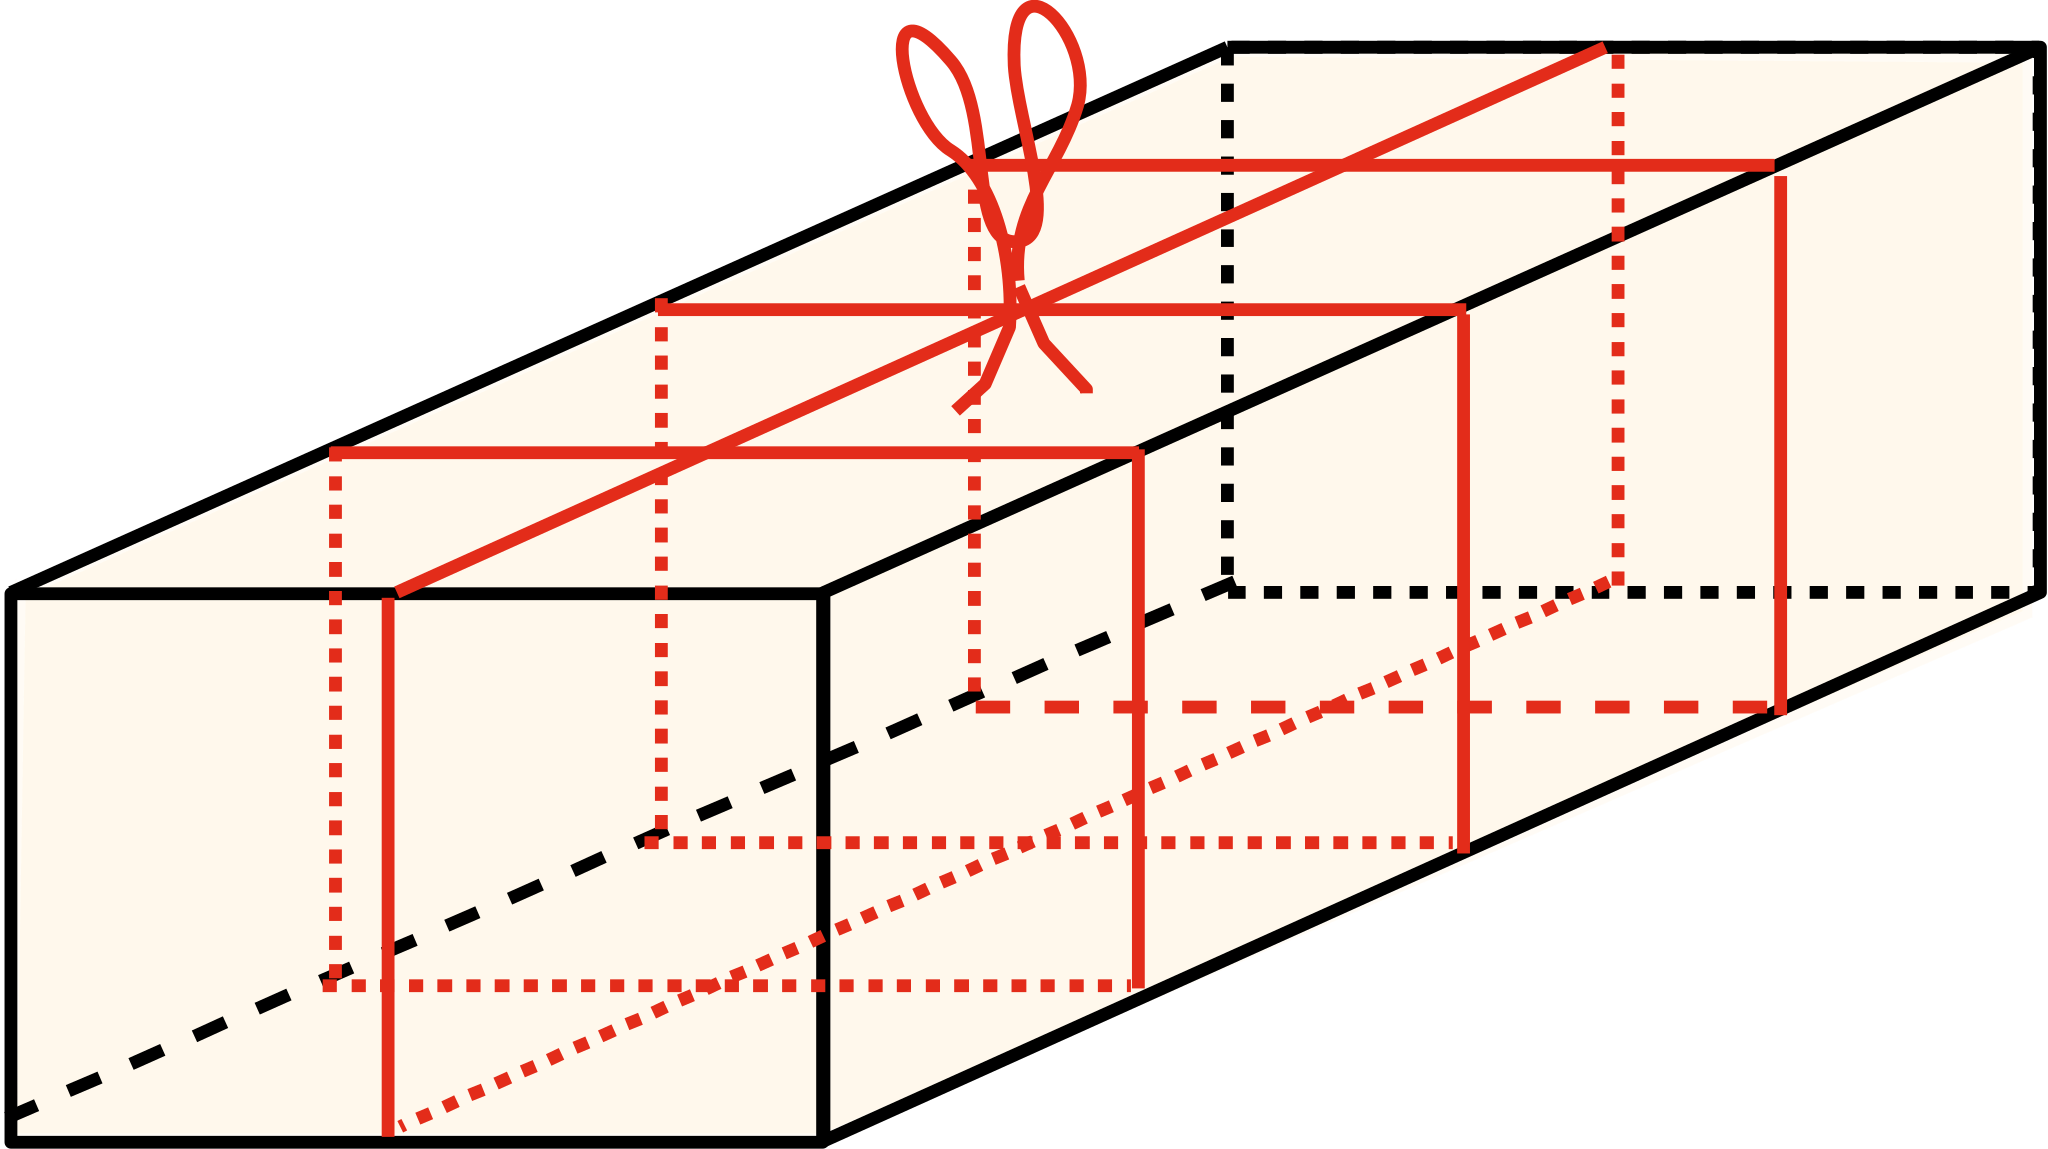
\includegraphics[width=3.1cm]{pelote2} \label{VolSol_entrain4}
 \end{colenumerate}
\begin{itemize}
 \item Pour chaque paquet, donne la longueur en mètres de ficelle utilisée par Mandy.
 \item Combien de paquets \ref{VolSol_entrain3} pourra‑t‑elle ficeler avec une pelote ?
 \item Combien de paquets \ref{VolSol_entrain4} pourra‑t‑elle ficeler avec deux pelotes ?
 \end{itemize}
\end{exercice}


%%%%%%%%%%%%%%%%%%%%%%%%%%%%%%%%%%%
%%%%%%%%%%%%%%%%%%%%%%%%%%%%%%%%%%%
%MiseEnPage
%%%%%%%%%%%%%%%%%%%%%%%%%%%%%%%%%%%
\newpage
%%%%%%%%%%%%%%%%%%%%%%%%%%%%%%%%%%%
%%%%%%%%%%%%%%%%%%%%%%%%%%%%%%%%%%%

%%%%%%%%%%%%%%%%%%%%%%%%%%%%%%%%%%%%%%%%%%%%%%%%%%%%%%%%%%%%%%%%%%%%%%

\serie{Patrons}

\begin{exercice}[Patrons d'un cube ?]
Quels dessins représentent un patron de cube ? 
\begin{colenumerate}{3}
 \item
 
 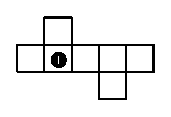
\includegraphics[width=2.4cm]{patron_cube1}
 \item
 
 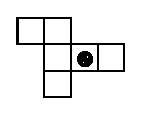
\includegraphics[width=1.9cm]{patron_cube2}
 \item
 
 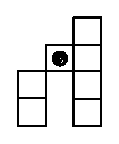
\includegraphics[width=1.5cm]{patron_cube3}
 \item
 
 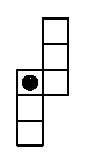
\includegraphics[width=0.9cm]{patron_cube4}
 \item
 
 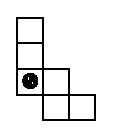
\includegraphics[width=1.4cm]{patron_cube5}
 \item
 
 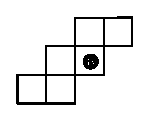
\includegraphics[width=2.05cm]{patron_cube6}
 \end{colenumerate}
\end{exercice}


\begin{exercice}[Patron et pavé]
Soit une représentation en perspective cavalière et un patron d'un pavé droit :

\begin{minipage}[c]{0.48\linewidth}
 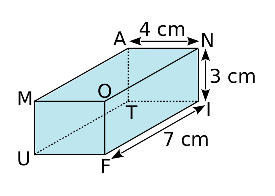
\includegraphics[width=4.3cm]{patron_pave}
 \end{minipage} \hfill%
 \begin{minipage}[c]{0.48\linewidth}
  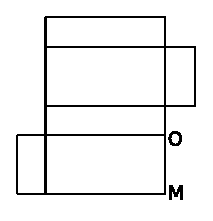
\includegraphics[width=3.105cm]{patronOM}
  \end{minipage} \\
\begin{enumerate}
 \item Reproduis, à main levée, le patron du pavé droit ; complète le nom des sommets et code les égalités de longueurs. 
 \item Trace ce patron en vraie grandeur.
 \end{enumerate}
\end{exercice}


\begin{exercice}[Patrons d'un pavé ?]
Quels dessins représentent un patron de pavé droit ? Justifie.

\begin{minipage}[c]{0.48\linewidth}
 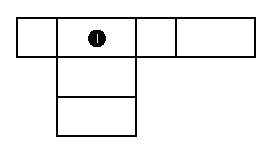
\includegraphics[width=4.2cm]{patron_pave1}
 \end{minipage} \hfill%
 \begin{minipage}[c]{0.48\linewidth}
  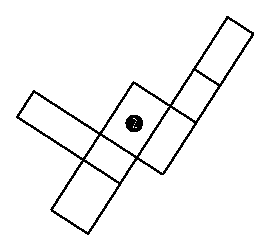
\includegraphics[width=4.1cm]{patron_pave2}
  \end{minipage} \\
\begin{minipage}[c]{0.3\linewidth}
 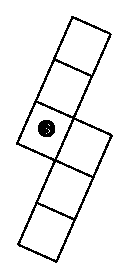
\includegraphics[width=1.7cm]{patron_pave3}
 \end{minipage} \hfill%
 \begin{minipage}[c]{0.33\linewidth}
  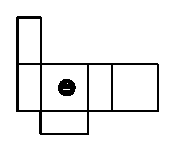
\includegraphics[width=2.5cm]{patron_pave4}
 \end{minipage} \hfill% 
 \begin{minipage}[c]{0.34\linewidth} 
  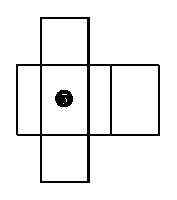
\includegraphics[width=2.5cm]{patron_pave5}  
  \end{minipage} \\
\end{exercice}


\begin{exercice}[Au choix]
\begin{minipage}[c]{0.68\linewidth}
Associe ce pavé droit à son patron. Justifie.
 \end{minipage} \hfill%
 \begin{minipage}[c]{0.30\linewidth}
  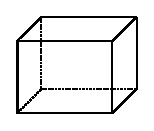
\includegraphics[width=2.1cm]{pave_simple}
  \end{minipage} \\
\begin{minipage}[c]{0.48\linewidth}
  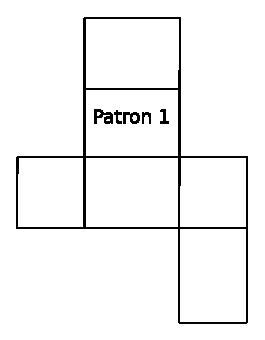
\includegraphics[width=4.1cm]{choix_patron1}
 \end{minipage} \hfill%
 \begin{minipage}[c]{0.44\linewidth}
  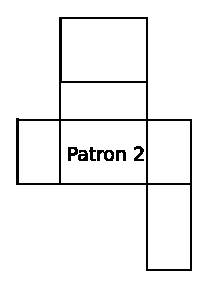
\includegraphics[width=3.1cm]{choix_patron2}
  \end{minipage} \\
\end{exercice}


\begin{exercice}
Reproduis, à main levée, chaque patron de pavé droit en complétant les longueurs manquantes :
\begin{minipage}[c]{0.58\linewidth}
  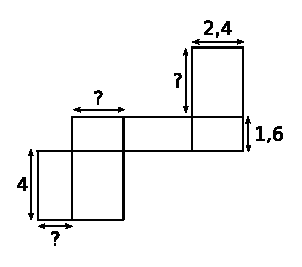
\includegraphics[width=4.7cm]{patron_completer1}
 \end{minipage} \hfill%
 \begin{minipage}[c]{0.38\linewidth}
  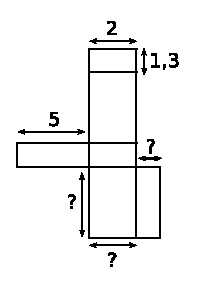
\includegraphics[width=2.8cm]{patron_completer2}
  \end{minipage} \\
\end{exercice}

%%%%%%%%%%%%%%%%%%%%%%%%%%%%%%%%%%%
%%%%%%%%%%%%%%%%%%%%%%%%%%%%%%%%%%%
%MiseEnPage
%%%%%%%%%%%%%%%%%%%%%%%%%%%%%%%%%%%
\newpage
%%%%%%%%%%%%%%%%%%%%%%%%%%%%%%%%%%%
%%%%%%%%%%%%%%%%%%%%%%%%%%%%%%%%%%%

\begin{exercice}[Patrons en vrac]
Recopie puis complète chaque patron de pavé droit :
\begin{center} 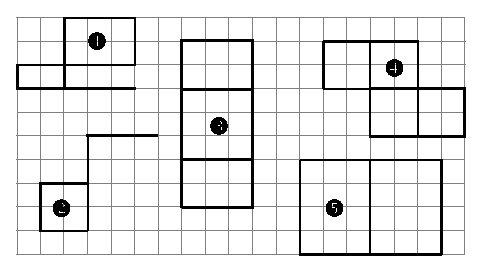
\includegraphics[width=8cm]{patron_pavedroit} \end{center}
\end{exercice}


\begin{exercice}
Trace un patron des solides dont les dimensions sont dans les tableaux ci‑dessous :
\begin{enumerate}
 \item
 
 \begin{center}
  \renewcommand*\tabularxcolumn[1]{>{\centering\arraybackslash}m{#1}}
  \begin{ttableau}{\linewidth}{4}
  \hline
  \rowcolor{C3} Pavé droit & Longueur & Largeur & Hauteur \\\hline
  \cellcolor{C3} \circled{1} & 4,5 cm & 2 cm & 6 cm \\\hline
  \cellcolor{C3} \circled{2} & 27 mm & 1,5 cm & 42 mm \\\hline
  \cellcolor{C3} \circled{3} & 5,3 cm & 25 mm & 74 mm \\\hline
  \end{ttableau}
  \end{center}
 \vspace{0.5cm}
 \item
 
 \begin{center}
  \renewcommand*\tabularxcolumn[1]{>{\centering\arraybackslash}m{#1}}
  \begin{ttableau}{\linewidth}{2}
  \hline
  Cube & Longueur de l'arête \\\hline
  \circled{4} & 4,5 cm \\\hline
  \circled{5} & 56 mm \\\hline
  \end{ttableau}
  \end{center}
 \end{enumerate}
\end{exercice}


\begin{exercice}
\begin{minipage}[c]{0.66\linewidth}
\vspace{1cm}
Réalise un patron de ce cube d'arête 3,6 cm sachant que les motifs sur deux faces opposées sont identiques.
 \end{minipage} \hfill%
 \begin{minipage}[c]{0.28\linewidth}
\vspace{1cm}
  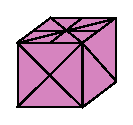
\includegraphics[width=1.7cm]{paquet_rose}
  \end{minipage} \\
\end{exercice}


\begin{exercice}
\begin{minipage}[c]{0.46\linewidth}
\vspace{1.9cm}
Réalise un patron de ce pavé droit composé de trois cubes identiques d'arête 2 cm, en respectant les couleurs.
 \end{minipage} \hfill%
 \begin{minipage}[c]{0.46\linewidth}
 \vspace{1cm}
  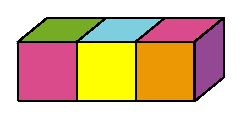
\includegraphics[width=3.4cm]{3cubes_colores}
  \end{minipage} \\
\end{exercice}


%%%%%%%%%%%%%%%%%%%%%%%%%%%%%%%%%%%
%%%%%%%%%%%%%%%%%%%%%%%%%%%%%%%%%%%
%MiseEnPage
%%%%%%%%%%%%%%%%%%%%%%%%%%%%%%%%%%%
\columnbreak
%%%%%%%%%%%%%%%%%%%%%%%%%%%%%%%%%%%
%%%%%%%%%%%%%%%%%%%%%%%%%%%%%%%%%%%

%%%%%%%%%%%%%%%%%%%%%%%%%%%%%%%%%%%%%%%%%%%%%%%%%%%%%%%%%%%%%%%%%%%%%%

\serie{Calculer des volumes}

\begin{exercice}[Volume par comptage]
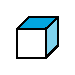
\includegraphics[width=0.7cm]{unite_volume} est 1 unité de volume.

 Donne le volume de chaque solide en unités de volume. Les volumes sont supposés pleins.
\begin{colenumerate}{2}
 \item
 
 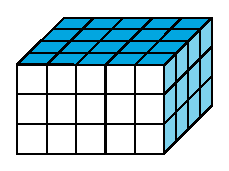
\includegraphics[width=3.4cm]{unite_volA} 
 
 \item
 
 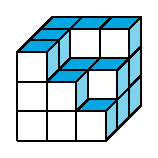
\includegraphics[width=2.2cm]{unite_volB} 
 
 \item
 
 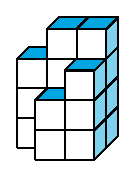
\includegraphics[width=1.8cm]{unite_volC} 
 
 \item
 
 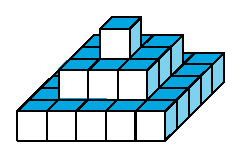
\includegraphics[width=3.7cm]{unite_volD} 
 
 \item
 
 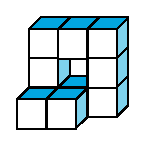
\includegraphics[width=1.8cm]{unite_volE} 
 \end{colenumerate}
\end{exercice}


\begin{exercice}[Volume de pavés]
Recopie le tableau et calcule les valeurs de $a$, $b$, $c$, $d$, $e$ et $f$ :
\begin{center}
 \begin{tabularx}{\linewidth}{|c|*{4}{>{\centering\arraybackslash}X|}}
 \hline
 & \cellcolor{H2} Longueur & \cellcolor{H2} Largeur & \cellcolor{H2} Hauteur & \cellcolor{H2} Volume \\\hline
 \cellcolor{U1} $P_1$ & \cellcolor{H3} 3 cm & \cellcolor{H3} 1 cm & \cellcolor{H3} 2 cm & \cellcolor{H3} $a$ \\\hline
 \cellcolor{U1} $P_2$ & \cellcolor{H3} 3,5 mm & \cellcolor{H3} 2 mm & \cellcolor{H3} 1 mm & \cellcolor{H3} $b$ \\\hline
 \cellcolor{U1} $P_3$ & \cellcolor{H3} 2,2 dm & \cellcolor{H3} 8 cm & \cellcolor{H3} 3 dm & \cellcolor{H3} $c$ \\\hline
 \cellcolor{U1} $P_4$ & \cellcolor{H3} 6 dm & \cellcolor{H3} 5 dm & \cellcolor{H3} $d$ & \cellcolor{H3} 120 dm\up{3} \\\hline
 \cellcolor{U1} $P_5$ & \cellcolor{H3} $e$ & \cellcolor{H3} 4 m & \cellcolor{H3} 3,2 m & \cellcolor{H3} 74,24 m\up{3} \\\hline
 \cellcolor{U1} $P_6$ & \cellcolor{H3} 2,5 hm & \cellcolor{H3} 2,7 dam & \cellcolor{H3} $f$ & \cellcolor{H3} 81 dam\up{3} \\\hline
 \end{tabularx}
 \end{center}
\end{exercice}

%%%%%%%%%%%%%%%%%%%%%%%%%%%%%%%%%%%
%%%%%%%%%%%%%%%%%%%%%%%%%%%%%%%%%%%
%MiseEnPage
%%%%%%%%%%%%%%%%%%%%%%%%%%%%%%%%%%%
\newpage
%%%%%%%%%%%%%%%%%%%%%%%%%%%%%%%%%%%
%%%%%%%%%%%%%%%%%%%%%%%%%%%%%%%%%%%

\begin{exercice}[Des solides]
Calcule le volume de chaque solide constitués de parallélépipèdes rectangles :
\begin{colenumerate}{2}
 \item 
 
 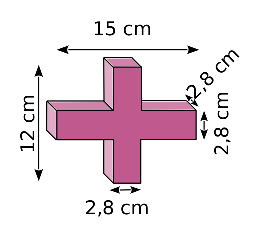
\includegraphics[width=3.8cm]{croix_rose}
 \item 
 
 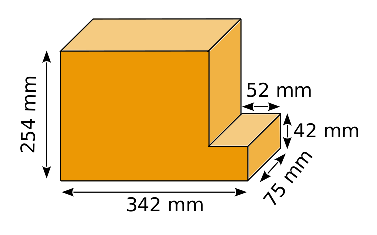
\includegraphics[width=5.5cm]{marche_orange}
 \item 
 
 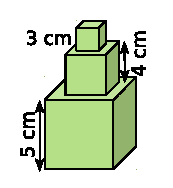
\includegraphics[width=2.5cm]{pile_verte}

 \end{colenumerate}
\end{exercice}


\begin{exercice}[Attention aux unités]
\begin{enumerate}
 \item Un cube de côté 1,2 m est percé de part en part par un trou fait à partir d'un carré de côté 12 cm. Calcule le volume du solide obtenu : \\[0.3em]
 \begin{center} 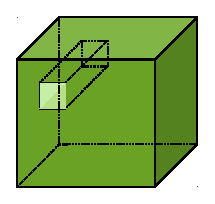
\includegraphics[width=3.2cm]{double_cube} \end{center}
 \item Calcule en cm\up{3} le volume de ce solide : \\[0.3em]
 \begin{center} 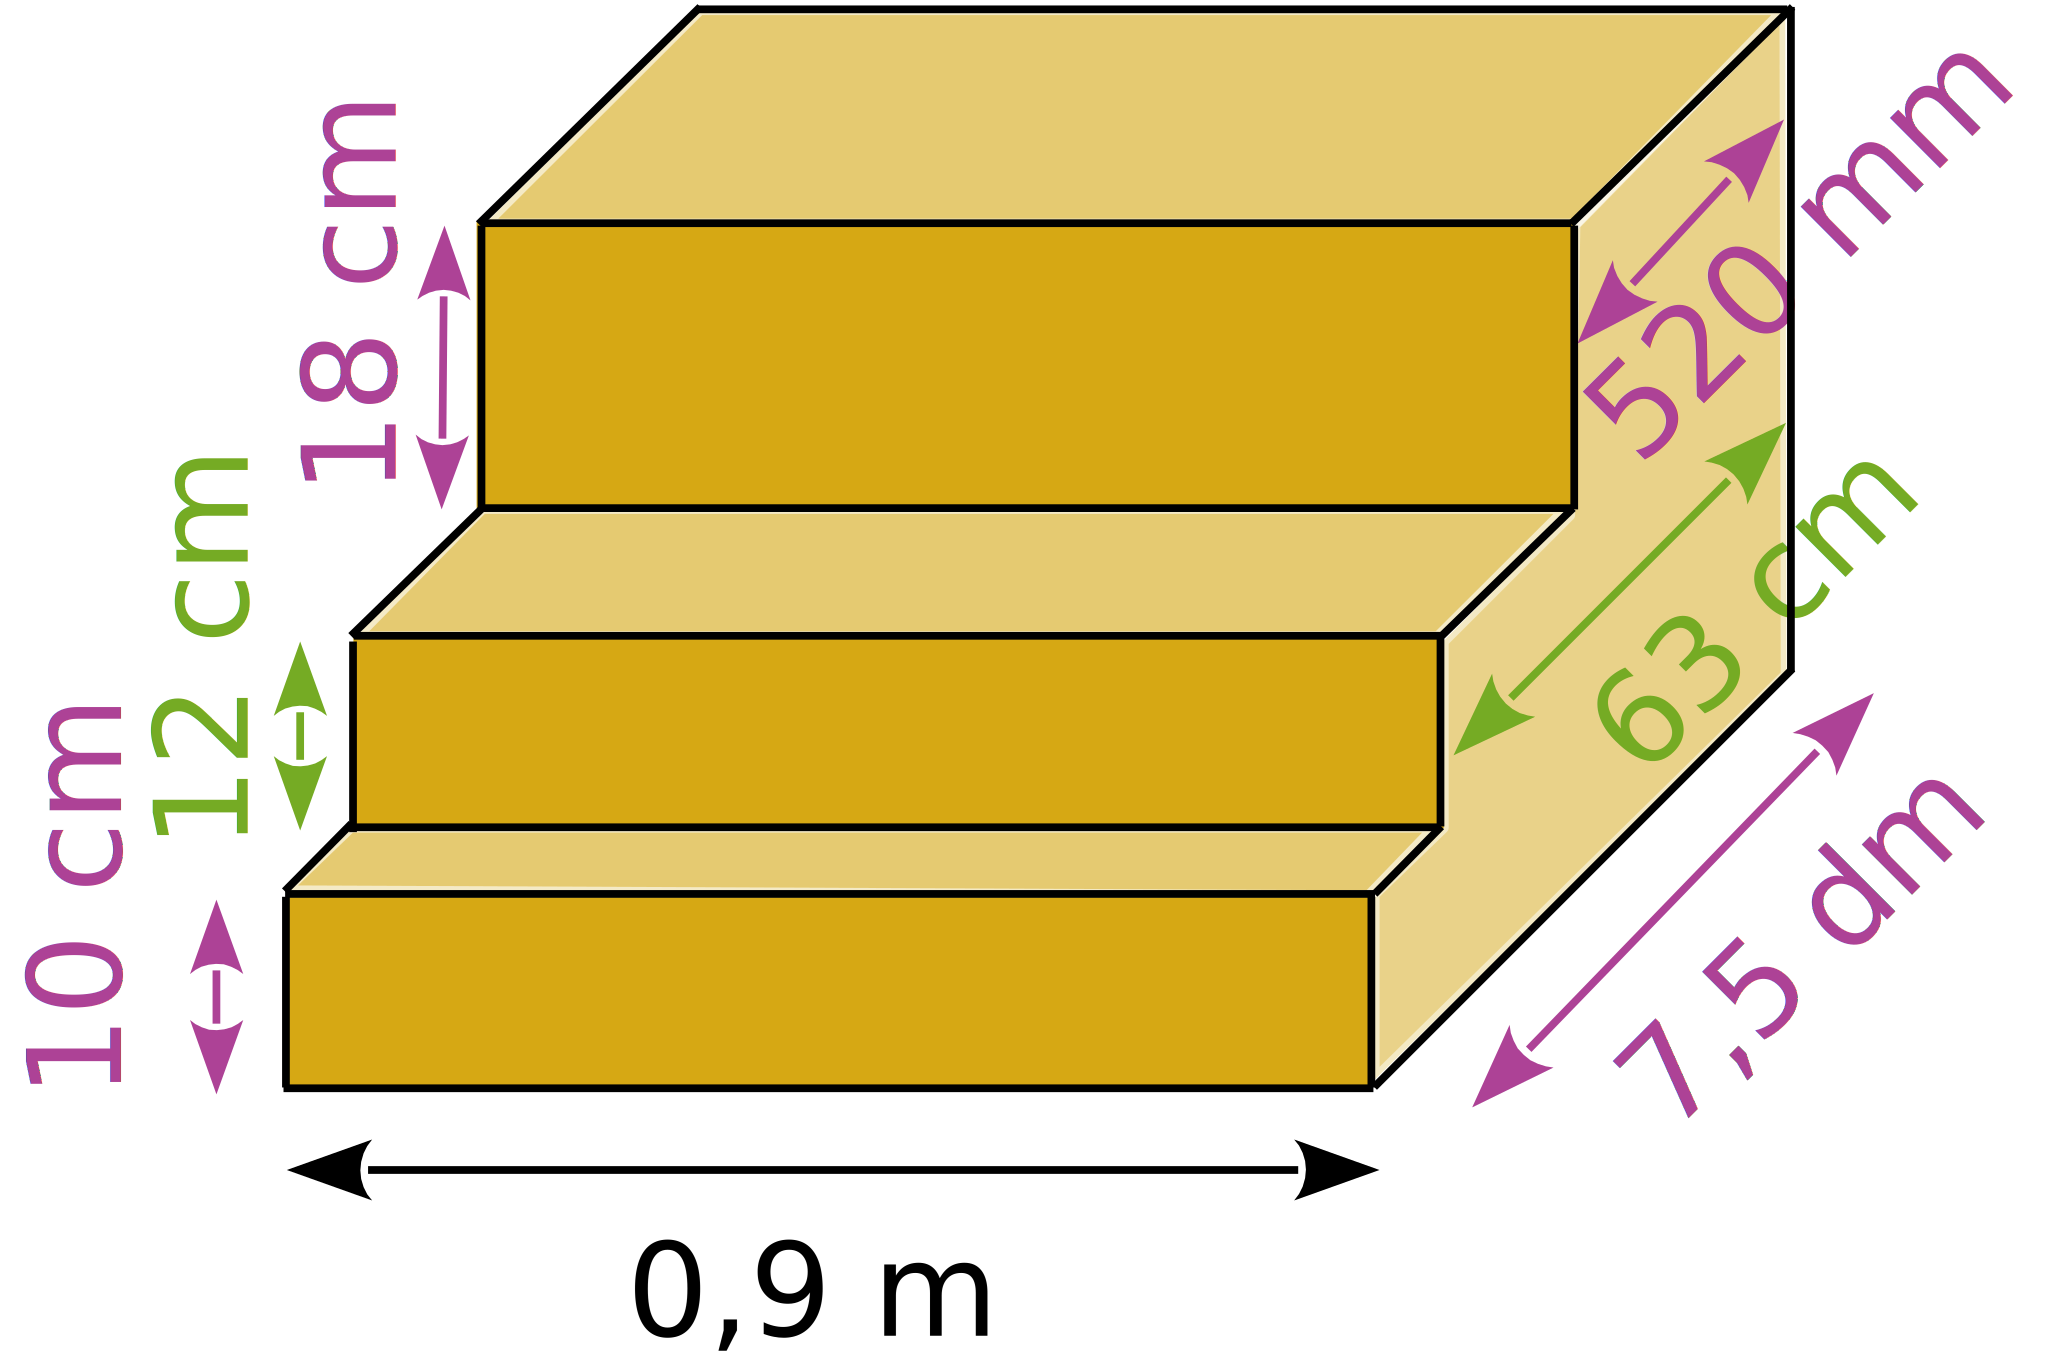
\includegraphics[width=5cm]{3marches} \end{center}
 \end{enumerate}
\end{exercice}


\begin{exercice}[Des tables]
Une table est composée d'un plateau rectangulaire de 3 cm d'épaisseur qui mesure 1,3 m de long et 0,8 m de large. Les pieds ont une base carrée de 9 cm de côté et une hauteur de 72 cm. \\[0.3em]
 \begin{center} 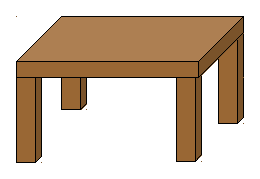
\includegraphics[width=5cm]{table_brune} \end{center}
 \begin{enumerate}
  \item Calcule le volume de bois nécessaire pour fabriquer cette table.
  \item Le chêne qui constitue cette table a une densité d'environ 0,7, ce qui signifie qu'un mètre cube de chêne pèse 700 kg. Combien pèse cette table si on la construit en chêne ?
  \item Une autre table construite en ébène (densité = 1,10) a une masse de 60,5 kg. Quel est le volume de cette table ?
  \end{enumerate}
\end{exercice}

